\documentclass[12pt]{article}
%\usepackage{hyperref}
\usepackage{natbib}
\bibpunct[: ]{(}{)}{;}{a}{}{,}
\usepackage[left=1.15in, right=1.15in, top=1in, bottom=1.25in]{geometry}
\usepackage{graphicx}
\usepackage{url}
\usepackage{booktabs}
\usepackage{lscape}
\usepackage{subfig}
\usepackage{setspace}
\usepackage{comment}




\begin{document}
\title{The Stratification of Culture Talk\footnote{Previous versions of this paper were presented at colloquia at the University of Notre Dame and at the MIT/Harvard Economic Sociology Seminar series. I would like to thank Roberto Fernandez, Robert Fishman, Gene Halton, Mary Ellen Konieczny, Elena Obukhova and Ezra Zuckerman for helpful comments on earlier drafts.  Direct correspondence to Omar Lizardo, University of Notre Dame, Department of Sociology, 810 Flanner Hall, Notre Dame, IN, 46556  Tel: (574) 631-1855, Fax: (574) 631-9238, Email: \ttfamily{olizardo@nd.edu}.}}
\author{Omar Lizardo \\ \textit{University of Notre Dame}}

\maketitle
\begin{center}
Words: 10,827
\end{center}•

\newpage
\newpage
\begin{center}
	{\large The Stratification of Culture Talk}
\end{center}

\begin{abstract}
\small In this paper, I explicitly characterize and establish the substantive relevance of a phenomenon that is crucial in connecting cultural inequalities to stratification outcomes:  namely, ``culture talk,'' or the use of conversational content associated with popular culture and the arts in face-to-face interaction with friends and acquaintances.  I argue that this phenomenon---central to many \emph{theories} of the connection between culture and stratification---deserves more \emph{empirical} attention.  To begin to bridge this gap, I analyze survey data from a probability sample of Americans to the first time document the socio-demographic correlates of culture talk.  The results show that the frequency of culture talk across five culture consumption domains is stratified according to the traditional markers of socio-economic status (such as levels of schooling and income) net of self-reported culture-consumption frequency, that the highly educated are more likely to engage in culture talk than the lower educated at comparably (high) levels of consumption and that consumption of in traditionally high status domains (the fine arts) is a better predictor of culture talk across all domains than consumption in less status stratified domains.  
\end{abstract}
\newpage
\newpage
\doublespacing
\newpage
\section{Introduction} 
Empirical research at the intersection of the sociology of culture and stratification has been primarily concerned  with exploring inequalities linked to social position in \emph{access} to and \emph{engagement} with symbolic goods  \citep{katzgerro04}.  The primary question in this burgeoning literature is whether taste and culture consumption patterns---as constitutive of the lifestyles that mark Weberian status groups---continue to be associated with social position \citep{tomlinson03}.  This organizing concern can be appreciated whether the construct of ``social position'' is conceptualized in terms of educational attainment \citep{ warde_etal08}, membership in broadly defined occupational groups \citep{tomlinson03}, aggregate measures of social class \citep{katzgerro06}, or constructed scalar indices of social status based on patterns of interaction (e.g. inter-marriage) across occupational groups \citep{chan_goldthorpe07a}. 

The main conclusion of this still vibrant line of research is that lifestyle practices continue to be strongly shaped---albeit in increasingly complex ways---by social position however it is defined \citep{bennett_etal08}.  One basic finding is now well-established:  members of the educated, salaried-professional elite are more likely to actively appropriate a wider variety of aesthetic offerings, within and across industry-defined genre categories and institutional contexts of dissemination and reception \citep{peterson05, warde08, lizardo08, prieur_savage11}. In essence, what it means to be high-status in contemporary societies is to be an equal opportunity connoisseur of diverse cultural offerings and aesthetic experiences across domains (e.g. literature versus film, and within domains across substyles), forms of delivery (e.g. non-profit versus commercial systems) and external legitimation (e.g. ``prescribed'' or ``authorized'' culture versus ``pop culture'', ``folk culture'' or ``kitsch'') \citep{peterson_kern96, bennett_etal08, prieur_savage11}.
	
This set of findings run counter to the predictions of ``postmodernization'' and class ``destructuration'' theorists who foresaw an inexorable decline in (and ultimate elimination of) the link between social position and lifestyle in market-dominated ``consumer societies''\citep[e.g.][]{pakulski_waters96}. In direct contrast to this claim, culture and stratification scholars can confidently assert that generalized markers of social status and education (rather than social class more narrowly defined) provide the best lens to understand cultural stratification patterns in the current context, confirming the basic findings of an earlier generation of research \citep{dimaggio_useem78a}. 

\subsection{What is good taste good for?}
The persistent focus of the cultural stratification literature on the question of \emph{whether} lifestyle practices continue to be unevenly segmented according to class and status markers has resulted in a relative lack of attention to an equally important question:  what is the \emph{role} (or ``function'') of aesthetic consumption in the everyday lives of members of different social strata? More precisely, \emph{given} the highly educated and those who belong to high-prestige occupational groups are more likely to engage with and be more generally knowledgeable about popular culture and the arts, how is this knowledge implicated in everyday behavior?  In essence, now that we know that eclecticism is the form that ``good'' taste takes in contemporary societies, it is time to ask---with \citep{erickson91}---``what is [this kind of] good taste good for''?

This gap in our knowledge is surprising in light of the fact that the status of popular culture and the arts as a form of \emph{class culture} was, and continues to be, central to the theoretical tradition from which most analysts of the culture-stratification build on in the first place \citep{collins75, dimaggio87, douglas_isherwood96}.  In this respect, Gary Alan Fine's basic complaint about research of popular culture in the early 1970s---that this research generally ignored the \emph{behavioral implications} of everyday engagement with culture and the arts especially as it pertains to face-to-face interaction \citep[453]{fine77}---can be repeated vis a vis research on cultural stratification today.  

One of the key analytic lessons of some of the foundational writings in the culture and stratification literature is that general familiarity with a given class culture is useful symbolic resource when it can be used as a signal providing an entry-point into delimited arenas of association \citep{mohr_dimaggio95}.  This is the reason why, in their influential paper, \citet{lamont_lareau88} linked the notion of cultural capital to an explicit conceptual framework that highlighted the active deployment of a given repertoire of cultural tastes and lifestyle practices for the purposes of drawing symbolic boundaries.  \citet{dimaggio87} was also adamant---building on the early work of Collins \citeyearpar{collins75}---in proposing that the major differences across status groups in the role that engagement with symbolic goods play in everyday social settings is connected to the \emph{routine exploitation of cultural knowledge in social interaction within everyday settings} \citep{erickson96, lizardo06a}. From this perspective, one substantively important way that the set of cultural aptitudes and interests characteristic of upper-middle class lifestyles become actualized as cultural \emph{capital}---that is ``convertible'' into other resources \citep{bourdieu86}---is through the linkage of cultural engagement to everyday processes of informal socialization and thus status group reproduction in the Weberian sense \citep{dimaggio_mohr85}.


\subsection{Culture talk as sociability}
We can begin to characterize the empirical phenomenon will be the focus of analysis via the rather common observation that conversational rituals usually require some sort of \emph{content} for their successful initiation and maintenance \citep{dimaggio87, collins75}. Whenever the primary conversational subject matter animating a given interaction episode moves towards the arts and the symbolic products of the culture industry, we may consider this an instance of  \emph{culture talk}. Following this lead, I define culture talk as \emph{the (more or less) routine deployment of cultural knowledge associated with aesthetic goods as a resource to generate conversation}. In a nutshell: the discussion of ``cultural matters'' with friends and acquaintances.

From a Simmelian perspective, we may consider culture talk one of the primary examples of ``sociability'' in late modern societies. Sociability is social interaction that is not driven by explicit instrumental purposes, but that is keyed to the continuing repetition of episodes of social interaction for their own sake \citep{simmel49}. Sociability thus represents the limiting case---and because seemingly devoid of explicit purpose, the ``play form''---of the more general process of association (coming together from some purpose).  In this respect, sociability is a \emph{form} of social intercourse explicitly dissociated from any sort of goal-directed pursuit. As a social form, sociability is thus partially independent of the particular content that drives it in a given context, making culture talk a fairly general (and generic) phenomenon.  However, this partial independence of form from content does not mean that just any content will do.

\subsubsection{The importance of aesthetic discourse as content}
Recent theorizing on the culture-network link has moved beyond the early formalism of traditional network analysis to propose that specifying the form of association is not enough; instead, particular forms of association are constituted by specific cultural contents that provide meaning to those forms \citep{fuhse09}.  Here I propose that in the contemporary context talk related to (1)  \emph{aesthetic consumption experiences} \citep{holbrook_hirschman82, deighton92, gainer95}, and (2) general knowledge of the accepted discursive conventions governing expressions of aesthetic categorization, evaluation and enjoyment \citep{baumann07, frith98} become one of the most important sources of meaningful content making possible sustained episodes of sociability.

As Simmel noted, sociability cannot be driven by traditional ``practical'' contents (e.g. work, politics, etc.), but requires instead ludic content that serves to simply sustain the focus of attention in the interaction itself \citep{collins75}. The reason for this is that sociability is a kind of social intercourse ``which does not have a strictly economic or business purpose'' but access to which (and restrictions on) is a key marker of the status group boundaries \citep[114]{weber94}---although in other contexts similar kinds of seemingly purposeless content are useful in \emph{relaxing} those same status boundaries \citep{ikegami05}. Building on Simmel, I argue that culture talk is the primary manifestation of sociability in contemporary class-differentiated societies, precisely because conversation related to symbolic goods is the ideal ludic content that fits this form of interaction. In comparison to aesthetic talk other types of conversational content---such as for instance religion or politics---are miserable failures, because they tend to suppress conversation and tend to highlight latent social divisions \citep{eliasoph98}.

Where does aesthetic content come from? Cultural theorists have persuasively argued that media-culture and arts dissemination institutions play a key role in producing an overabundant supply of (sometimes ephemeral) content useful for generating discussion that serves as a resource for conversation in the context of small groups  \citep[453]{fine77}.  The recurrently reproduced micro-orders based on face-to-face (and increasingly electronically mediated) interaction require a constant stream of novel content in order to be recurrently recreated and thus reproduce themselves over time. 

In this respect, the formal and informal system of production of aesthetic goods provide as ``input'' the very content that serves as the scaffolding around which everyday episodes of ``talk'' and sociability are built.  Popular culture scholars have proposed that ``[p]art of the pleasure of popular culture is talking about it; part of its meaning is{\ldots}talk''  \citep[4]{frith98}. Accordingly, civic membership and even ``belonging'' to neighborhoods and communities is partially constituted via talk, and ``[m]uch of this talk is about the mass media and its cultural commodities'' \citep[73]{fiske87}. For instance, Elizabeth Long \citeyearpar{long03} in her study of women's reading groups in Houston, Texas, finds that cultural knowledge and taste become the primary content of social interaction. Consistent with the claim that connects the consumption of aesthetic products and sociability, she finds that reading group members ``tend to press books into service for the meanings that they transmit and the conversations they generate \citeyearpar[73]{long03}. Simlarly, \citet[316-317]{benzecry_collins14} point to the crucial role of culture talk in constituting the aesthetic experience for fanatics of Opera in Buenos Aires. Among Opera fans, talk is almost constant, and this talk revolves around the music, past performances, and tales of their own ``heroic commitment'' to the art form. Through this talk Opera fanatics ritually construct and maintain their relationship to other fans, while at the same time marking the boundary separating true connoisseurs from less serious followers. 

Why is aesthetic talk effective at relationship building and maintenance? As noted in both classic \citep{fine77, dimaggio87} and more recent work \citep{cardon_granjon05, lewis_etal12}, talk about culture and the arts infuses local conversation-based interaction rituals with a common focus of attention, serving as fodder for either deep, engrossing conversations \citep{frith98} or ``for least-common denominator talk'' \citep[443]{dimaggio87}, depending on the pragmatic context. In contrast to material goods which ``are physically present and visible'' and which may serve as barriers for interaction via the creation of invidious distinction, the consumption of aesthetic goods ``\ldots is invisible once it has occurred. This evanescent quality makes artistic experience, described and exploited in conversation, a portable and thus potent medium of interactional exchange.'' \citep[443-444]{dimaggio87}. Because commercial (``popular'') culture and the arts (along with ``fashion, cuisine and sport'') are the closest analog to a common cultural currency in contemporary societies \citep{dimaggio00a}, they have the capacity to be a smooth facilitator of interaction across situational settings, social occasions and social positions\citep{erickson96}. 

Both early \citep{dimaggio87, fine77} and more recent \citep{long03, benzecry_collins14} considerations of the role of culture talk in the creation and maintenance of social relations via consumption and interaction rituals, converges with work in marketing and consumer culture studies \citep{deighton92, gainer95}. According to \citet{gainer95}, art consumers use conversation about the arts to make what could potentially be a purely private experience part of their public interactions with others. Via culture talk, persons con-construct both their own personal identities as art consumers \emph{and} their interpersonal relations with other art aficionados. In this way, ``social relationships are often created and maintained through rituals of reproduction based on consumption which individuals join in shared performances with symbolic meaning.''\citep[254]{gainer95}. Consumption of the arts, as mediated via culture talk, allow persons to pursue interpersonal goals connected to companionship and friendship, build bridges to socially distant acquaintances, generate interaction rituals for work conversation \citep{lizardo13}, establish criteria for co-membership in exclusive social circles \citep{kadushin66}, while at the same time managing and reinforcing individual and community identities \citep[255-257]{gainer95}. 


\subsection{The stratification of culture talk}
The Simmelian formulation that equates culture talk with sociability, while revealing, also obscures a fact that is relatively uncontroversial for contemporary theorists of the culture/stratification link.   Rather than simply being a formal or neutral ``form'' of association, opportunities to engage in the type of non-instrumental sociability that Simmel points to is not likely to be equitably distributed in the social structure.  The reason for this is precisely that access to practical familiarity with the content in question is itself inequitably distributed \citep{bourdieu84}. This type of ``conversation for enjoyment'' \citep[124]{collins75}, \emph{precisely} because it is dissociated from explicit instrumental pursuits and because it is not driven by ``extrinsic rewards'' but by friendship and personal liking, comes to serve as one of the primary ways in which vertical and horizontal status-group boundaries are dynamically built and re-built.  These boundaries are recurrently recreated mainly via processes of inclusion and exclusion at the interactional level. 

Accordingly, when the very knowledge and associated experiences that are required for engaging in this form of interaction are unequally distributed \citep{reay10}---coming to form the basis for the formation of partially segregated status cultures  \citep{bourdieu84}---then we should find that members of high-status groups should be more likely to routinely engage in culture talk.  One obvious reason for this comes from what is the basic finding of the sociology of taste:  there continue to exist strong socio-demographic differences in rates of familiarity and engagement with culture and the arts, especially across groups defined by such status markers as education (and to a lesser extent, income) \citep{bennett_etal08}.  If aesthetic experiences are translated into culture talk in mundane conversational settings, then we should expect that individuals who have a higher-baseline probability of of engagement and general familiarity with culture and the arts should also be more likely to engage in culture talk.  A strong version of this argument would predict that status-linked differences in the likelihood of engaging in culture talk are purely a product of differences in cultural engagement. Under this model, status-linked differences in cultural engagement are the primary source of individual differences in cultural knowledge.  Therefore, there should not exist any residual differences across status groups \emph{within} levels of consumption.  In statistical terms, the direct effect of socio-economic status on culture talk is fully mediated by consumption frequency.

However, several considerations lead us to expect that this last version of the argument is not on the right track.  First, persons endowed with large stocks of cultural capital should be able to participate in conversation featuring culture as a topic even when they are not active consumers in the domain in question. That is, they may demonstrate what \citet[252]{peterson92} has referred as ``passing knowledge'' of a given cultural domain on the spot.  This is in fact a form of ``social skill'' that is almost a requirement among members of the young, highly-educated, new middle class \citep{dimaggio96}.   

Consistent with this hypothesis, current research on the culture-stratification link suggests that the ability to deploy cultural knowledge in interaction in partial dissociation from direct consumption is generated via multiple routes:  (1) past experience in the educational system---``scholastic capital'' in Bourdieu's \citeyearpar[59]{bourdieu84} sense---where traditional high-status culture (and increasingly ``popular'' culture) have become established part of the curriculum, (2) past experience in the upper-middle and middle-class household---``domestic capital'' in Bourdieu's \citeyearpar[59]{bourdieu84} sense---where extra-curricular forms of aesthetic engagement and arts-training have become an institutionalized element of the socialization process; (3)  routine interaction with members of the personal network who are themselves avid consumers of the cultural forms in question and who thus make culture talk a recurrent conversational topic allowing ego to gather cultural knowledge that may be used in other conversational interactions \citep{cardon_granjon05}; and finally, (4) person-to-organization connections that allow high-status individuals to participate in elite urban social circles where culture talk is a prescribed conversational resource \citep{ostrower98}.

This alternative conceptualization of the link between culture talk and social position suggests the existence of (relatively) strong structuration of culture talk by socio-economic status and other markers of difference, even after adjusting for the relative propensity to directly participate in the cultural realms in question.  These residual socio-demographic differences in culture talk propensities should be strongest precisely across those social markers most clearly associated with status and privilege, such as education and income stratum.\footnote{As noted by \citet{bennett_etal08}, this does not imply that those persons who are disengaged from cultural consumption do not have active social lives. My argument \emph{does} imply however, that the social lives of the aesthetically disengaged will be structured in distinct ways, by for instance being relatively more tied to neighborhood and locality \cite{prieur_savage11}.}   However, insofar as mechanisms associated with network connectivity and social capital may also be involved in generating the capacity to participate in ``interaction rituals''  featuring culture talk (independent of consumption), other axes of difference partially orthogonal to socio-economic status---but correlated with social connectivity---should retain their predictive power even after adjusting for levels of cultural consumption \citep{collins04}. 

Nevertheless, we should not expect all dimensions of socio-economic status to be equally good predictors of culture talk. As argued above, culture talk is deeply tied to a person's capacity to appropriate cultural goods and then mobilize discursive resources related to those consumption experiences in interaction. In this respect, culture talk is more closely connected to a given person's stock of (embodied) \emph{cultural capital} than it is to economic resources. Accordingly, we should find that those dimensions of socio-economic status that more closely track a history of accumulation of cultural capital (such as educational qualifications) should be better predictors of culture talk than those dimensions of socio-economic status that index material advantage (such as income).

\begin{quote}
Hypothesis 1:  \emph{A person's socio-economic status predicts culture-talk  frequency even after adjusting for levels of cultural participation.}
\end{quote}

Insofar as being an active participant in the arts is a clear index of cultural capital, a variation of this argument would propose that the differences in cultural talk propensities that are traceable to differences in socio-economic status themselves not independent from a person's status as an active arts participant. Instead we should expect that the predictive power of socio-economic status should change depending on whether we are talking about active or inactive culture-consumers. More specifically we should expect that status-linked differences in the likelihood of engaging in culture talk should be larger among active culture-consumers than among inactive ones.  This would be consistent with a world in which even when exposed to a similar set of experiences, persons would not only differ in the capacity to translate those experiences into a conversational resource based on social location, but this differential capacity should be most evident among persons who are more likely to engage in culture consumption in the first place.  This is consistent with a \emph{cumulative advantage} mechanism \citep{diprete_eirich06} linking consumption, status position and culture talk.  If this is correct, members of the high status groups should not only be more likely to engage in culture talk than their lower-status counterparts but this difference should be largest among the most active consumers.

\begin{quote}
Hypothesis 2:  \emph{Socio-economic status is a better predictor of culture talk frequency for culturally active persons.}
\end{quote}

\subsection{Cross-domain differences}
Does the stratification of culture talk vary across domains?  The fact that the traditional fine arts dissemination institutions, such as galleries and museums, symphony orchestras and theaters, continue to be patronized mainly by a highly selected, educated elite is a well-established empirical finding \citep{dimaggio_mukhtar04}.  We also know that attempts to ``democratize'' access to the fine arts on the part of these institutions have met with equivocal results, and in most cases have failed outright \citep{alexander96}.  The dependence of non-profit arts organizations on this consumer base provides high-status elites with recurrent occasions to meet others in the same circles at sponsored social gatherings \citep{ostrower98}.  These are interaction opportunities that are ideally suited for the deployment of culture talk.  

In addition, it is clear that the field of fine arts production possess a long-standing legacy of discursive tools---developed by professional critics and lay enthusiasts---for the critical evaluation and the \emph{intellectualized} expression of taste judgments \citep{weber77}.  The availability of established linguistic conventions with which to categorize and evaluate cultural products may facilitate the mobilization of this type of content as a conversational resource among high-status elites \citep{dimaggio87}.  In all, if we presume that routine access to and knowledge about the visual and performance arts is certainly more strongly stratified by education and socio-economic status than is the case for more commercialized domains, then we should find that culture talk involving this type of content should also be more highly stratified by status.

\begin{quote}
Hypothesis 3: \emph{Socioeconomic status is a better predictor of culture-talk frequency in fine arts domains in comparison to commercial arts domains.}
\end{quote}

Recent studies of the consumption of the popular arts, inspired by Bourdieu's \citeyearpar{bourdieu93a} work on ``fields of cultural production,'' has begun to conceive of the popular and commercial arts as equally capable of being the subject of attempts to impose hierarchies of value and taste, the construction of exclusionary canons, and the establishment systems of cultural currency as the fine arts. Rather than operating according to a logic that is antithetical to that which structures fine arts consumption fields (as presumed by an earlier generation of popular culture studies, the realm of commercial culture production and consumption comes to be structured according to hierarchies of perception and evaluation that are premised upon categories of perception and vocabularies of appreciation developed in autonomous fields of cultural production to the products of the culture industry.  In this respect, ``artistic hierarchies, which rank producers according to their aesthetic or expressive value{\ldots}are becoming a central structuring force in a growing number of fields of production'' including that of rock and roll, a quintessential instance of the commercial arts \citep[98]{regev94}.  

More recently, other authors have begun to extend this analysis of the dynamics whereby other popular culture fields-such as film---come to acquire a hierarchical form modeled on the artistic field \citep[e.g.][]{allen_lincoln04}. Thus, as \citet{baumann01} has argued, certain commercial forms (such as film) have developed an intellectualized vocabulary of appreciation that matches that of their fine arts counterparts. The adoption of this ideology of autonomous art by producers and gate-keepers of the popular arts mirrors the increasing propensity of  (culturally advantaged) consumers of popular culture to adopt a similar stance \citep{thornton96}. 

Just like in the fine arts field, where struggles to define artistic value based on what is defined as `art' and `not art' are constantly in play, ``a similar use of accumulated knowledge and discriminatory skill is apparent in low cultural forms, and has the same hierarchical effect.  Low culture, that is to say, generates its own capital---most obviously perhaps, in those forms{\ldots}which are organized around  exclusiveness, but equally significant for the fans:{\ldots}of even the most inclusive forms'' \citep[9]{frith98}. Insofar as the popular arts are subject to this intellectualization process, and insofar as critical gatekeepers develop a language of appreciation and historical canonization, then they will be likely to figure as fodders for culture talk among high-status classes. Thus, in the very same way in which both the commercial and the traditional arts can be appropriated ``aesthetically'' by members of high status classes \citep{peterson_kern96}, we should find that high status groups are equal opportunity culture talkers across domains:

\begin{quote}
Hypothesis 4:  \emph{Socioeconomic status predicts culture-talk frequency across all cultural domains.}
\end{quote}

If culture talk is spurred by the extent to which a person is familiar with intellectualized discourses of cultural appreciation, then we should also expect that there should exist predictable \emph{asymmetries} in the extent to which the consumption of fine arts spurs cultural talk in commercial domains as opposed to the reverse. More specifically, we should find that the consumption of the fine arts (as an index of familiarity with the discursive conventions of art) should be an equally good predictor of culture talk in so-called commercial domains as the consumption of commercial art, but not vice versa. That is, fine arts consumers should be as (or more) likely to engage in culture talk in commercial domains, but commercial arts consumers should be less likely than fine arts consumers to engage in culture talk in fine arts domains:

\begin{quote}
Hypothesis 5:  \emph{Fine arts consumption is a better predictor of culture talk across both commercial and fine arts domains than commercial arts consumption.}
\end{quote}


\section{Analysis}
\label{sec:analysis}

\subsection{Data and Variables}
\label{subsec:data}

\subsubsection{Data Source}

In the empirical analysis that follows, I consider data obtained from the Arts and Culture Supplement to the National Social Survey fielded in 2002 ($N=1,002$) and 2004 ($N=801$) \citep{NSS2002, NSS2004}.  The NSS is a weighted (by age, education, marital status, gender, race, ethnicity) probability sample of respondents residing the United States collected through computer-aided telephone interviews.   The NSS is particularly appropriate for my purposes because both waves contain information not only about culture consumption experiences, but also about the likelihood that individuals engage in informal social interaction featuring cultural content taken from consumption in the same domains.  Because the items of interest were fielded in both waves, I pool individuals for which I have complete data on all socio-demographic variables from the 2002 ($N=1002$) and 2004 ($N=801$) surveys, resulting in a total combined sample of 1,803 respondents.

\subsubsection{Key response and control variables}
As part of the survey, respondents were asked to report (during the past twelve months), ``approximately how often have you had a discussion with someone you know'' about (1) a movie, (2) a musical performance, live or recorded, (3) a book, a poem or a story, (4) an art show or a work of art, and (5) a play or other dramatic performance.  These are the main empirical indicators of culture talk and thus will serve as the response variables in the analyses that follow.  Respondents were also asked to report how often (in the last year) they had been to the movies, listened to recorded music at home, read a book, had gone to an art show or a museum, or had gone to any live performances.  Because I am interested in accounting for residual socio-demographic differences in culture talk net of consumption, these serve as the main control variables in the analysis.  For both sets of responses, respondents were asked to choose from the following response categories: 1) very often, 2) fairly often, 3) not very often, 4) or not at all.\footnote{How does the NSS compare to other Arts participation Surveys?  When it comes to book reading, the 2002 NSS estimates that about 55.7\% of respondents report reading books ``Fairly Often'' or `` Very Often.''  The corresponding estimate for the 2002 SPPA (Survey for Public Participation in the Arts) is about 58\%.  When it comes to going to an art museum, about 12\% of NSS respondents report going ``Fairly Often'' and about 3.7\% of respondents report going ``Very Often''; these correspond well with SPPA 2002 data based on more specific questions on attendance frequencies:  13.4\% of SPPA respondents report having gone to the museum between 2 and 5 times in the last year, and 3.2\% report having gone more than five times.  In the NSS, about 9\% of respondents report going to a live performance ``Very Often.''  In the 2002 SPPA about 7.3\% of respondents report having gone out to a Jazz, Classical, Opera, Musical, Ballet or Dance performance between 2 and 5 times in the last year.  In all, the NSS appears to do a good job of capturing rates of arts participation that are comparable to that obtained from other National Surveys.}
 
\subsection{Analytic Strategy}
\subsubsection{Propensity of culture talk}
As noted above, one obvious answer to the question of the socio-demographic structuration of culture talk suggests that this outcome should be most strongly predicted by culture-consumption. Insofar as it is direct experiences with cultural goods and performances that come to serve as the source-content for culture talk episodes we should expect that individuals who are active culture consumers should also evince a higher propensity to engage in culture talk. However, my main interest is status-linked differences in culture talk propensity that are not directly traceable to diversity in consumption behavior.  Thus, I specify an ordered probit model \citep{long_freese06} that holds constant self-reported consumption frequency (as given by the above indicators), in order to ascertain whether there is residual variation across status groups (defined by levels of education) in culture talk propensity \emph{within-levels} of self-reported consumption.  This model takes the form:

\begin{equation}
E(P[Y_{it} \leq k])= \alpha_k + \gamma_t E_i + \delta_t C_{it} + \sum_k\beta_{kt}X_{ik} 
\label{eq:eq1}
\end{equation}•

Where $Y_{it}$ is the frequency of culture talk for individual $i$  in the $t^{th}$ cultural domain, $E_{i}$ is the educational attainment of that person, $C_{it}$ is the self-reported consumption frequency for each individual in that domain.  The effect of these last two  variables expected to be large and positive (and $\gamma_t>0$ and $\delta_t>0$). Finally, $\beta_k$ is an $i \times k$ vector of coefficient estimates corresponding to the effect of the other predictors included in the model ($X_{ik}$); this is the \emph{additive model}.  If there is residual status-linked variation in culture talk net of consumption then we should expect that $\gamma \neq 0$, after holding constant $W_{it}$.  

Alternatively, we may expect that the status effect should itself vary according to the level of self-reported consumption.  This would be the case, for instance, if persons of high-education engage in culture talk at higher rates than persons of low-education even when they consume culture at the same rates. I examine the validity of this hypothesis by specifying a model of the form:

\begin{equation}
E(P[Y_{it} \leq k])= \alpha_k + \gamma_t E_i + \sum_{j=2}^{4}  \delta_{jt} C_{ijt} + \sum_{j=2}^{4} \rho_{jt} C_{ijt}E_{ij} + \sum_k\beta_{kt}X_{ik}
\label{eq:eq2}
\end{equation}•

This is the \emph{multiplicative} model. In this model I enter the frequency of consumption as (4-1=3) binary indicators ($C_{ijt}$) and interact each with the education variable. As \citet{ai_norton03}, have recently noted, the empirical validity of hypothesis 2---which says that the effect of education varies across self-reported consumption status---cannot be verified simply by looking at the \emph{t}-statistics corresponding to each of the $\rho_{jt}$ effects. This is due to the fact that in non-linear (e.g. logit or probit) models the actual interaction effects depend on the value of all other variables in the model any may be present even if $\rho_{jt}=0$. Instead, after estimating the model, I compute the marginal effect of moving from the lowest to the highest education level on the probability of engaging in culture talk ``very often.''  I then graph the corresponding point estimate and 90\% confidence interval across groups of respondents defined by self-reported frequency levels.  The presence of a statistically discernible upward trend in the marginal effects estimates would constitute positive evidence of the expected interaction between status and frequency on consumption for that domain. 

\subsubsection{Indicators of socio-economic status}
I estimate five ordered probit models (one for each cultural domain) of the additive and multiplicative form with the culture talk indicator as the response variable, a series of socio-demographic variables as the predictor variables and the frequency of consumption for that cultural domain as the main control variable. The predictors were chosen  using a combination of criteria geared towards substantive relevance and predictive power. I was also limited by the availability of socio-demographic indicators in the survey: for instance, the NSS contains no information on respondent's current occupation or family background (both of which are theoretically relevant dimensions of social differentiation). 

The main indicator of socio-economic status, as indicated above, is educational attainment and, secondarily, family income.  The education variable is coded as five ordered categories (from high-school dropout to graduate or professional degree) and the income variable is coded in six ordered categories (from less than 20K a year to 100K or more).\footnote{Family income information was not available for about one fifth of the cases (20.8\%) across the two survey waves.  For these cases ($N=375$) I imputed their income using the multiple imputation procedure in Stata 11.  Essentially this involves using an ordered probit model to predict the missing income values using all remaining socio-demographic information for that respondent (e.g. education, age, marital status and selected interactions.} 

\subsubsection{Additional socio-demographic predictors}
The models presented below also include the following vector of socio-demographic covariates:  (1) respondent's age (in seven ordered categories),  (2) respondent's gender, and (3) urban Location (urban versus other location).  I experimented with models that included a vector of dummy variables coding for race/ethnic identification and marital status.  These variables had for the most part non-statistically significant effects in all of the equations.  To avoid over-parameterizing the models and for the sake of parsimony, I excluded these variables from the presentation of the results. Tables showing the coefficient estimates and t-statistics for these variables are available upon request from the author.  Descriptive statistics corresponding to each of the predictor variables included in the models are presented in Table~\ref{tab:desc} of the Appendix.  

For the sake of efficiency, simplicity, and to achieve comparability in the magnitude of the effects across the different types of predictors in the presentation of the results, I enter all of the ordered categorical predictors as numeric inputs into the various equations (summarizing the effect of education, for instance, in a single coefficient rather than ($K-1$ indicator variables, where $K$ is the number of ordered categories).  This linearity constraint results in some loss of information, but the substantive story remains the same regardless of the strategy I pursue (results available on request).  To facilitate comparison of the magnitude of the effects across inputs, I standardized each of the predictors by subtracting the mean and dividing by two times the standard deviation as recommended by \citet{gelman08}.  This makes the interpretation of  the (ordered categorical) numeric predictors such as education, income, and age straightforward: the coefficient estimate indicates the effect of moving from the lowest to the highest value, while the binary predictors (gender, urban and marital status) retain their usual interpretation.



\section{Results}
\subsection{Status-linked differences in the frequency of culture-talk}
Table~\ref{tab:talk-tab1} shows the point estimates and associated $t$-statistics corresponding to the predictors of expected self-reported frequency of culture talk across all five domains. Hypothesis 1 predicts that a person's socio-economic status should predict culture talk even after adjusting for participation frequency. The results are consistent with this hypothesis. Looking at the effect of education, I find that there exist strong levels of status-linked heterogeneity in culture-talk even after holding constant self-reported consumption behavior. Persons who have attained advanced educational qualifications are more likely to engage in culture talk featuring popular culture and the arts as content than persons who have not, within levels of self-reported participation frequency. The results are also consistent with the claim that when it comes to culture talk, education is the more relevant status characteristic (in comparison to income). In contrast to education, income is only a statistically significant predictor of culture talk in three out of the five models, and the substantive strength of the effect is comparatively weaker.

\subsection{Heterogeneity in the Education Effect Levels of Participation}
How does the additive model compare to the multiplicative specification?  Figure~\ref{fig:educgraph} shows the effect of education on the marginal probability of engaging in culture ``very often'' for respondents partitioned according to the levels of self-reported consumption in that domain. The strength of the multiplicative interaction between education and consumption can be gauged by the extent to which we observe any trends in the marginal effect estimate. The estimates are obtained from ordered probit models specified according to equation~\ref{eq:eq2}. 

Hypothesis 2 predicts that the education effect should be more pronounced among culturally active persons.  The results provide fairly strong levels of support for this hypothesis. Upward trends in the effect of education on inducing frequent levels of culture talk are clear in film book-reading, and to a lesser extent music.  They are much weaker in the case of dramatic performances. In the case of the visual arts, I simply find a categorical distinction between the most active participants and everybody else, with education-based differentiation in culture talk being strong for the former group and non-existent for the latter.  In all, these results provide fairly broad support for the hypothesis that status linked differences in culture talk are much stronger for the most active culture consumers.

\subsection{Heterogeneity in the Socio-Economic Status Effect Across Cultural Domains}
Hypothesis 3 predicts that status-based differentiation should be stronger for the traditional high-status cultural domains, while hypothesis 4 predicts that we should find status-based differentiation in all domains.  A quick glance at the pattern of results shown in table~\ref{tab:talk-tab1} reveals that, when it comes to education, hypothesis 4 is on the right track. The education advantage in culture talk is comparably strong across all cultural domains. 

\subsection{Culture Talk Differences Across Commercial and Fine Arts Audiences}
Hypothesis 5 says that fine arts consumers should be as likely to engage in culture talk in commercial domains than commercial domain consumers. In order to test this hypothesis I proceed in two steps. First, I create two variables designed to tap the relative likelihood of each respondent to engage in the commercial and fine arts. These variables come from a principal factor analysis of the five consumption frequency items, in which I retain only the two main factors (those with an eigenvalue larger than 0.9). I use a promax rotation to allow the factors to be correlated with one another. The factor loadings for the first two principal factors are shown in~\ref{tab:fac-tab}. As we would expect reading, visiting museums and galleries and loading to the theater load on a common factor, while going to the movies and listening to the music load on a second factor. The regression-based scores from these two factors are taken as indicators of the relative likelihood to engage the fine and commercial arts respectively.

In a second step, I introduce these two variables as predictors of culture talk in an ordered probit model that adjusts for the same variables as those shown in table~\ref{tab:talk-tab1}. The coefficient estimates for these models are shown in table~\ref{tab:talk-tab2} (I omit the presentation of the other estimates for the sake of simplicity). To test the hypothesis that fine arts consumption is a better predictor of culture talk than commercial arts consumption across all domains, I estimate a constrained model that forces these two coefficients to be the same. I then use a likelihood ratio test to check whether there is a significant loss of model fit in comparison to the unconstrained model. The results provide strong support for hypothesis 5. Across all domains except for film, being a fine arts consumer is a better predictor of culture talk ($p<0.05$). 
\section{Discussion}
\label{sec:discussion}
\subsection{Contributions}
This paper furthers current understandings of the mechanisms connecting culture and status group stratification by bringing attention to the socio-demographic correlates of an important phenomenon.  The literature on culture stratification has been primarily focused on the question of the determinants of lifestyle consumption patterns, with a view to establishing whether there still exists a correlation between cultural choices and social position.  This one-sided concern has led to the neglect of an equally important question: that of the behavioral implications of familiarity and engagement with the arts.  In this respect current research has generally failed to consider the existence of stratification-linked differences in the extent to which cultural knowledge is differentially ``put to use'' by members of different social strata as a resource for interaction \citep{dimaggio87, deighton92, gainer95, benzecry_collins14}.  To answer to this question, I synthesized insights from classical theoretical sources in the culture and stratification literature with recent empirical and conceptual advances in our thinking of the relationship between culture and social networks.  I argued that one of the most important behavioral implications of familiarity with culture and the arts is its role as the type of content that is useful for the generation of conversational interaction; in short, \emph{culture talk}.  This is a phenomenon that deserves as much empirical and theoretical attention the ``patterns of cultural choice'' \citep{peterson83} that have traditional monopolized the attention of culture and stratification researchers.   

This paper contributes to the study of culture and stratification in several ways: analytically, I developed a framework that partially meets my self-imposed challenge by highlighting the theoretical and empirical importance of the culture talk phenomenon. I began with the Simmelian legacy on the importance of seemingly ``purposeless'' (non-instrumental and non-goal-oriented) conversational content for the emergence of ``sociability'' (or the ``play form'' of association) and connected it to the more contemporary stress by cultural stratification theorists on ``entertainment talk'' as the cement that holds status groups together as micro-relational communities of acquaintance and informal membership \citep{collins75, dimaggio87, gainer95, purcell07, lizardo06a, rivera12}. Empirically, I advance research in the growing literature linking taste, lifestyle consumption and stratification. I do this by examining the socio-demographic structuring of culture talk as a constitutive component of lifestyle-based stratification in contemporary societies. The results  show that, consistent with prior theory in cultural stratification, culture talk is stratified by the same markers of social position and status that previous research has shown also characterize audience segmentation in the corresponding cultural domains. More specifically, I show that culture talk in all domains---whether commercial or the fine arts---is stratified by education, income, age and gender, and to some extent urban location \emph{net} of self-reported engagement in those domains.  Those individuals endowed with larger stocks of economic (members of the middle and upper classes) and cultural capital (the highly educated) are more likely to routinely engage in culture talk, the young are more likely to engage in culture talk than the old,  women are more likely to engage in culture talk than men, and urbanites (in some domains) are more likely to engage in culture talk than their suburbanite/rural-dwellers counterparts.   

\subsection{Implications for the Study of the Culture/Network Link}
This paper also contributes to the emerging literature on the culture/network linkage \citep{fuhse09, pachucki_breiger10}.  This emerging line of theory and research  has coalesced around a critique of older styles of network research that followed Simmel in viewing structural form as separable from cultural content and mid-twentieth century British Social Anthropology in conceiving of cultural meaning as an epiphenomenon constituted by more ``concrete'' network relations and status positions  \citep{wellman88}.  Recent reconsiderations of the culture-network linkage have decisively moved beyond this received picture in demonstrating that culture and meaning are in fact constitutive of network ties and proposing a more balanced dynamic interplay between relational form and cultural content \citep{vaisey_lizardo10}.  Nevertheless, the relevance of this theoretical re-thinking for substantive research on the topic of cultural stratification is not yet clear (but see \citet{schultz_breiger10}).  This paper provides a concrete substantive application of these recent insights that clarifies the implications of this new literature for the issues that matter to cultural stratification researchers.   I propose that aesthetic consumption experiences are one of the key contents constitutive of important forms of network connectivity in contemporary societies \citep{dimaggio87}.  

This argument and the results reported in this paper have broader implications contemporary theory on the connection between culture, connectivity and structured inequality \citep{erickson08}.  In this respect, the type of routine deployment of cultural knowledge in concrete interaction that I have labeled as culture talk can be thought of as an important \emph{relational mechanism} \citep{tilly98, gross09}, linking inequalities in the propensity to use aesthetic content as a conversational resource to inequalities in relational outcomes associated to social connectivity and status-based boundaries. These long-standing inequalities in connectivity (both in terms of range and diversity) have been duly noted in the network literature \citep{lin99, erickson08}, but have yet to receive a satisfactory explanation.  Building on the results reported in this paper, it can be argued that different rates of engagement in culture talk provides a micro-interactional mechanism accounting for the dynamic persistence of cross-group inequalities on the major dimensions of social connectivity.

First, under the proposed account, individuals who have a larger propensity to engage in culture talk should also have an easier time during the relationship-formation process \citep{lazarsfeld_merton54}.  This is a plausible micro-mechanism that can help us to account for the existence stubborn status-linked inequalities social capital.  For instance, it is well-known that education has been \citep{marsden87} and continues to be \citep{lizardo06a, diprete_etal11} one of the best predictors of network size in the United States---and other national settings \citep{mollenhorst_etal11}---today.   The higher-educated are also more likely to engage in culture talk than the less-educated (within-levels of consumption), and thus they should also be more likely to routinely use this as an interactional resource to form new relationships \citep{fine77, dimaggio87}. The same can be said for those socio-demographic groups known to have smaller networks than average such as the less-educated elderly \citep{cornwell_etal08}.  Culture talk propensities decline with age for this group, consistent with the claim that rates of relationship formation underlie these differences.

Second, persons who belong to socio-demographic groups that exhibit a larger propensity to engage in culture talk should also tend to be embedded in status segregated networks.   Social ties that are partially constituted via culture talk retain this property because they are dynamically sustained via conversational meanings and contents access to which is also status-segregated \citep{collins75}.   In this respect, differential rates of culture talk across socio-demographic groups emerge as a plausible mechanism that accounts for the existence of status-segregated social networks even in the absence of any strictly conscious attempt on the part of individuals to select status-homogamous contacts.   

Third, it is well-established that the social-networks of Americans are characterized by high-rates of status-endogamy specially premised on race and education \citep{diprete_etal11}, and that marital homogamy premised on education and income has increased at the expense of marital endogamy premised on other axes of difference \citep{ kalmijn94, schwartz10}.  Persons who belong to high-education or high-income groups are also more likely to engage in culture talk than the less-educated (within-levels of consumption).  Following the same line of reasoning, they should also be expected to be more likely to routinely use this as an interactional resource to recurrently recreate status-segregated conversational rituals \citep{collins04, rivera12, nagel_etal11}.

Finally,  those individuals who have a more pronounced propensity to engage in culture talk should also tend to be more likely to bridge structural and ``cultural holes'' \citep{pachucki_breiger10, lizardo06a, lizardo11a}. This is a phenomenon that has been referred by \citet{schultz_breiger10}---riffing on \citet{granovetter73} and building on \citet{erickson96} and \citet{lizardo06a}---as \emph{the strength of weak culture}.  Status-linked inequalities in culture talk propensities can thus be proposed as a mechanism that explains the often noted fact that high-status individuals are more likely to be connected to a more diverse pool of others than low status individuals \citep{marsden87, erickson96, erickson08, lin_dumin86, lin99, goldstein_warren00, diprete_etal11}.   With persons of high education and/or high-income more likely to engage in culture talk than the less-educated, it stands to reason that they should also be able to---in some settings \citep{purcell07}---use this cultural expertise to make sporadic connections \emph{across} group and status boundaries.   

While the validity and scope of these hypotheses remains to be more fully explored, the results reported in this paper---along with convergent evidence from other sources \citep{lizardo06a, lizardo11a, lewis_etal09, rivera12, schultz_breiger10}---strongly point in this direction, suggesting exciting prospects for future research in this area.  In this manner, a focus on the culture talk phenomenon can serve to cross-fertilize research in the culture and stratification literature and the sociology of taste with research on inequalities in network access and social capital.  


\singlespacing
\newpage
\bibliographystyle{asr}
\bibliography{main}

\newpage
\begin{figure}[ht!]
\centering
\caption{Marginal effects of education on the probability of engaging in culture talk ``very often,'' by levels of cultural engagement in five cultural domains, 2002 and 2004 NSS.}
\label{fig:educgraph}
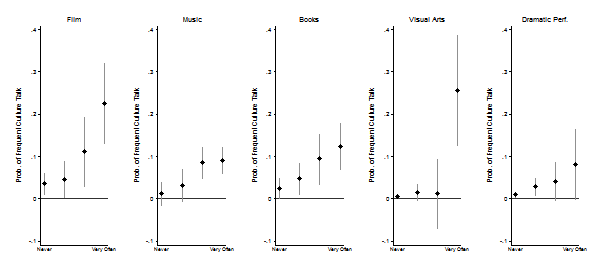
\includegraphics[width=6.5in]{educgraph.png}
\end{figure}•
%\newpage
\begin{table}[ht!]
	\caption{\small Coefficient Estimates for Predictors of Expected Frequency of Culture-Talk, Ordered Probit Estimates, 2002, 2004 NSS.}
	{
\def\sym#1{\ifmmode^{#1}\else\(^{#1}\)\fi}
\begin{tabular*}{\hsize}{@{\hskip\tabcolsep\extracolsep\fill}l*{5}{c}}
\toprule
                    &\multicolumn{1}{c}{Movies}&\multicolumn{1}{c}{Music}&\multicolumn{1}{c}{Books}&\multicolumn{1}{c}{Arts}&\multicolumn{1}{c}{Plays}\\
\midrule
main                &             &             &             &             &             \\
Education (centered)&        0.26*&        0.33*&        0.28*&        0.22*&        0.25*\\
                    &      (4.80) &      (5.97) &      (4.99) &      (3.63) &      (4.35) \\
Family Income (centered)&        0.08 &        0.17*&        0.10*&        0.07 &        0.18*\\
                    &      (1.48) &      (3.14) &      (1.91) &      (1.18) &      (3.19) \\
Age (centered)      &       -0.45*&       -0.27*&       -0.25*&       -0.16*&       -0.16*\\
                    &     (-8.11) &     (-5.18) &     (-4.72) &     (-2.86) &     (-3.03) \\
Gender (Woman=1)    &        0.23*&        0.06 &        0.33*&        0.19*&        0.27*\\
                    &      (4.32) &      (1.07) &      (6.18) &      (3.42) &      (5.12) \\
Urban Location (Yes=1)&        0.05 &        0.19*&        0.10*&        0.08 &        0.23*\\
                    &      (0.95) &      (3.62) &      (1.92) &      (1.46) &      (4.22) \\
Consumption Freq.   &        1.04*&        0.62*&        1.08*&        1.28*&        1.05*\\
                    &     (17.39) &     (11.29) &     (19.09) &     (21.60) &     (18.39) \\
\midrule
cut1                &             &             &             &             &             \\
Constant            &       -1.15*&       -0.70*&       -0.91*&       -0.13*&       -0.36*\\
                    &    (-28.94) &    (-21.11) &    (-24.97) &     (-4.17) &    (-11.26) \\
\midrule
cut2                &             &             &             &             &             \\
Constant            &       -0.31*&        0.13*&       -0.04 &        1.05*&        0.76*\\
                    &     (-9.55) &      (4.16) &     (-1.22) &     (27.10) &     (21.69) \\
\midrule
cut3                &             &             &             &             &             \\
Constant            &        0.71*&        1.00*&        0.79*&        1.85*&        1.61*\\
                    &     (20.83) &     (27.65) &     (22.80) &     (34.03) &     (34.03) \\
\midrule
Obs                 &        1791 &        1795 &        1792 &        1790 &        1793 \\
BIC                 &      4367.4 &      4724.7 &      4498.9 &      3634.9 &      4052.3 \\
Model $\chi^{2}$    &       568.7 &       266.4 &       529.5 &       609.6 &       517.8 \\
\bottomrule
\end{tabular*}
}

	\label{tab:talk-tab1}
	$*p<0.05$ (One-tailed test)
\end{table}

\newpage
\begin{table}[ht!]
	\caption{\small }
	{
\def\sym#1{\ifmmode^{#1}\else\(^{#1}\)\fi}
\begin{tabular*}{\hsize}{@{\hskip\tabcolsep\extracolsep\fill}l*{1}{ccc}}
\toprule
                    &    Factor 1&    Factor 2&      $\psi$\\
\midrule
How Often Read Books (for Pleasure)&       0.637&      -0.239&       0.610\\
How Often Went to Museums/Galleries&       0.783&      -0.105&       0.415\\
How Often Went to Live Performances&       0.650&       0.264&       0.426\\
How Often Listen to Music&      -0.091&       0.882&       0.252\\
How Often Went to Movies&       0.389&       0.458&       0.553\\
\bottomrule
\end{tabular*}
}

	\label{tab:fac-tab}
\end{table}

\newpage
\begin{table}[ht!]
	\caption{\small Coefficient Estimates for Selected Predictors of Expected Frequency of Culture-Talk, Ordered Probit Estimates, 2002, 2004 NSS.}
	{
\def\sym#1{\ifmmode^{#1}\else\(^{#1}\)\fi}
\begin{tabular*}{\hsize}{@{\hskip\tabcolsep\extracolsep\fill}l*{5}{c}}
\toprule
                    &\multicolumn{1}{c}{Movies}&\multicolumn{1}{c}{Music}&\multicolumn{1}{c}{Books}&\multicolumn{1}{c}{Arts}&\multicolumn{1}{c}{Plays}\\
\midrule
main                &             &             &             &             &             \\
Fine Arts Factor Score&        0.24*&        0.47*&        0.30*&        0.36*&        0.52*\\
                    &      (7.44) &     (15.47) &      (8.15) &      (7.80) &     (12.67) \\
Commercial Arts Factor Score&        0.18*&        0.26*&        0.17*&        0.04 &        0.11*\\
                    &      (5.60) &      (4.72) &      (5.48) &      (1.42) &      (3.41) \\
\midrule
Obs                 &        1780 &        1779 &        1778 &        1780 &        1781 \\
BIC                 &      4263.1 &      4385.8 &      4341.5 &      3553.7 &      3875.0 \\
Model $\chi^{2}$    &       653.4 &       577.8 &       663.0 &       684.7 &       681.8 \\
\bottomrule
\end{tabular*}
}

	\label{tab:talk-tab2}
	$*p<0.05$ (One-tailed test)
\end{table}



\newpage
\section*{Appendix}
\begin{table}[ht!]
	\caption{\small Coefficient Estimates for Predictors of Expected Frequency of Cultural Participation, Ordered Probit Estimates, 2002, 2004 NSS.}
	{
\def\sym#1{\ifmmode^{#1}\else\(^{#1}\)\fi}
\begin{tabular*}{\hsize}{@{\hskip\tabcolsep\extracolsep\fill}l*{5}{c}}
\toprule
                    &\multicolumn{1}{c}{Movies}&\multicolumn{1}{c}{Music}&\multicolumn{1}{c}{Books}&\multicolumn{1}{c}{Arts}&\multicolumn{1}{c}{Plays}\\
\midrule
main                &             &             &             &             &             \\
Education (centered)&        0.25*&        0.09 &        0.36*&        0.59*&        0.43*\\
                    &      (4.51) &      (1.52) &      (6.58) &      (9.83) &      (7.76) \\
Family Income (centered)&        0.28*&       -0.01 &        0.05 &        0.21*&        0.24*\\
                    &      (5.18) &     (-0.14) &      (0.99) &      (3.54) &      (4.46) \\
Age (centered)      &       -0.77*&       -0.60*&        0.10*&       -0.10*&       -0.22*\\
                    &    (-14.34) &     (-9.76) &      (1.87) &     (-1.73) &     (-4.23) \\
Gender (Woman=1)    &        0.12*&        0.17*&        0.36*&        0.10*&        0.04 \\
                    &      (2.37) &      (3.02) &      (6.93) &      (1.79) &      (0.70) \\
Urban Location (Yes=1)&        0.23*&        0.04 &        0.10*&        0.18*&        0.23*\\
                    &      (4.44) &      (0.64) &      (1.87) &      (3.14) &      (4.30) \\
\midrule
cut1                &             &             &             &             &             \\
Constant            &       -0.51*&       -1.70*&       -0.90*&        0.14*&       -0.34*\\
                    &    (-15.87) &    (-33.37) &    (-25.89) &      (4.47) &    (-10.91) \\
\midrule
cut2                &             &             &             &             &             \\
Constant            &        0.59*&       -0.99*&       -0.18*&        1.08*&        0.60*\\
                    &     (18.26) &    (-27.46) &     (-6.08) &     (28.92) &     (18.68) \\
\midrule
cut3                &             &             &             &             &             \\
Constant            &        1.33*&       -0.36*&        0.43*&        1.88*&        1.40*\\
                    &     (32.33) &    (-11.77) &     (13.95) &     (33.17) &     (32.90) \\
\midrule
Obs                 &        1792 &        1798 &        1795 &        1792 &        1794 \\
BIC                 &      4401.5 &      3603.4 &      4847.0 &      3715.8 &      4472.5 \\
Model $\chi^{2}$    &       280.5 &       106.5 &       108.9 &       163.8 &       150.2 \\
\bottomrule
\end{tabular*}
}

	\label{tab:freq-tab}
	$*p<0.05$ (One-tailed test)
\end{table}

\newpage

\begin{table}[ht!]\centering \caption{Descriptive statistic for predictor, control and response variables included in the analyses. \label{tab:desc}}
\begin{tabular}{l c c c c c}\hline\hline
\multicolumn{1}{c}{\textbf{Variable}} & \textbf{Mean}
 & \textbf{Std. Dev.}& \textbf{Min.} &  \textbf{Max.} & \textbf{N}\\ \hline
How Often Read Books (for Pleasure) & 2.719 & 1.126 & 1 & 4 & 1800\\
How Often Went to Museums/Galleries & 1.646 & 0.832 & 1 & 4 & 1797\\
How Often Went to Live Performances & 2.006 & 0.966 & 1 & 4 & 1799\\
How Often Listen to Music & 3.41 & 0.892 & 1 & 4 & 1803\\
How Often Went to Movies & 2.091 & 0.972 & 1 & 4 & 1797\\
How Often Discussed a Movie & 2.709 & 1.053 & 1 & 4 & 1801\\
How Discussed a Book Poem or Story & 2.553 & 1.099 & 1 & 4 & 1800\\
How Often Discussed a Play & 1.973 & 0.955 & 1 & 4 & 1802\\
How Often Discussed Art show Work & 1.797 & 0.908 & 1 & 4 & 1801\\
How Often Discussed a Musical Perf. & 2.38 & 1.055 & 1 & 4 & 1800\\
Education & 4.039 & 1.21 & 1 & 6 & 1800\\
Family Income & 3.345 & 1.779 & 1 & 6 & 1798\\
Age & 4.59 & 2.023 & 1 & 7 & 1799\\
Gender (Woman=1) & 0.5 & 0.5 & 0 & 1 & 1803\\
Urban Location (Yes=1) & 0.6 & 0.49 & 0 & 1 & 1803\\
\hline\end{tabular}
\end{table}



\end{document}